\section{Modeling and Simulation of Turbulent Combustion} % (fold)
\label{sec:simulation_of_turbulent_combustion}
%
Simulations are used to make predictions about the behavior of a system.
%
In turbulent combustion and other engineering application they provide a
quick and cheap way of testing setups compared to setting up experiments.
%
A simulation is only useful if it is sufficiently accurate.
%
This is why good models of the underlying processes are so important.
%
On the other hand, simulations also need to be efficient.
%
If running the simulation is more expensive and time-consuming than setting up
a comparable experiment, the simulation loses its value.
%

%
For turbulent combustion, finding a good trade-off between accuracy and
efficiency is very much an open problem.
%
Both turbulent flow and chemical reactions are complex to model and expensive
to simulate on their own.
%
Solving both at once in a turbulent combustion simulation predictably leads to
a vast increase in the required computing time and resources.
%
Frequently simplifying assumptions are made to gain efficiency.
%
Which assumptions are valid under which circumstances is the central question
when building turbulent combustion models.
%

%
This section provides an overview of modeling strategies used in turbulent
combustion simulations.
%
It places a particular focus on \acl{DNS}, as it is most relevant for the
content of this thesis.
%
\subsection{Chemical Schemes} % (fold)
\label{sub:chemical_schemes}
%
Modeling a chemical reaction can be a complex task.
%
Most reactions do not consist of a single step but rather a complex system of
intermediate reactions.
%
Many of these reactions can be reversible and their reaction rates depend on the
current composition and pressure or temperature of the gas.
%
The more complex the fuel, the more intermediate steps are possible and need to
be considered when modeling the reaction.
%
A system of intermediate steps that models a whole reaction is called a chemical
scheme (see, \eg, \cref{tab:hydrogen_scheme}).
%
Each individual reaction step has a number of parameters controlling the
reaction rate in dependence on the current conditions.
%
\begin{table}[t]
    \caption[Example scheme for \ce{H2}-\ce{O2} combustion]
            {Example scheme for a seemingly simple chemical reaction: hydrogen
             and oxygen react to produce water \cite{Miller1982}. \ce{M} is a
             placeholder for any third molecule that is needed to absorb and
             dissipate excess energy to stabilize the product.}
    \label{tab:hydrogen_scheme}
    \centering
    \begin{tabularx}{\linewidth}{lX}
    \toprule
    \textbf{Elements:} & \ce{H},  \ce{O},  \ce{N} \\
    \midrule
    \textbf{Species:} & \ce{H2}, \ce{O2}, \ce{OH}, \ce{O}, \ce{H}, \ce{H2O},
                        \ce{HO2}, \ce{H2O2}, \ce{N2}\\
    \midrule
    \textbf{Reactions:} &
    {$\begin{aligned}
        \ce{H2 + O2 &<=> 2 OH} & \ce{2 OH &<=> O + H2O}\\
        \ce{H2 + OH &<=> H2O + H} & \ce{H2 + M &<=> 2 H + M}\\
        \ce{H + O2 &<=> OH + O} & \ce{O2 + M &<=> 2 O + M}\\
        \ce{O + H2 &<=> OH + H} & \ce{H + OH + M &<=> H2O + M}\\
        \ce{H + O2 + M &<=> HO2 + M} & \ce{HO2 + H &<=> H2 + O2}\\
        \ce{H + 2 O2 &<=> HO2 + O2} & \ce{2 HO2 &<=> H2O2 + O2}\\
        \ce{H + O2 + N2 &<=> HO2 + N2} & \ce{H2O2 + M &<=> 2 OH + M}\\
        \ce{OH + HO2 &<=> H2O + O2} & \ce{H2O2 + H &<=> H2 + HO2}\\
        \ce{H + HO2 &<=> 2 OH} & \ce{H2O2 + OH &<=> H2O + HO2}\\
        \ce{O + HO2 &<=> O2 + OH} &
    \end{aligned}$}\\
    \bottomrule
    \end{tabularx}
\end{table}
%

%
Reaction modeling is the task of breaking down the wealth of possible
intermediate reactions into a subset that describes the whole reaction with
sufficient accuracy for a given application, and determining the right
parameters for each one.
%
For complex hydrocarbon fuels the number of different species considered
can easily go into the hundreds, while thousands of intermediate steps
contribute to the reaction.
%
Even for seemingly simple reactions, such as hydrogen and oxygen to water,
the reaction schemes can be surprisingly complex.
%
The scheme by Miller \etal{}~\cite{Miller1982} displayed in
\cref{tab:hydrogen_scheme} has 9 species and 19 different reversible reactions.
%
Adding this to an already computationally intensive fluid dynamics simulation
that only involves five different variables (density, temperature and three
velocity components) increases the computational load immensely.
%
This is amplified even more by the fact that chemical reactions, especially the
intermediate ones in a reaction scheme, typically happen at much smaller time
scales than the flow.
%
This means that compared to non-reacting flows, not only do the number of
equations and variables increase immensely, but the simulation time steps also
become much smaller.
%

%
There are some strategies to increase efficiency.
%
The simplest one is to use single-step chemistry.
%
Here, the reaction is assumed to be infinitely fast and the flame front to be
infinitely thin.
%
Fuel and oxidizer are immediately transformed into products and heat once the
conditions for combustion are met.
%
In this case, no intermediate reactions are considered, which greatly decreases
the number of variables and equations to solve and allows larger time steps.
%
Due to the strong assumptions made when using this method, the results can be
very inaccurate, but it can be useful to get a qualitative result.
%
More accurate but also more expensive methods precompute a lookup table covering
the relevant portion of the parameter space or reduce the parameter space to
lower-dimensional manifolds.
%
Explaining these methods in detail is out of the scope of this work.
%

%
Modeling chemical reactions is a complex field in its own right.
%
Turbulent combustion researchers mostly use existing chemical libraries and
schemes in their codes.
%
Often, the trade-off between accuracy and efficiency has to lean heavily towards
efficiency to keep simulation times and memory usage in a reasonable range.
%
% subsection chemical_schemes (end)
%
\subsection{The Flamelet Assumption} % (fold)
\label{sub:the_flamelet_assumption}
%
Moving from the modeling of reactions in an idealized uniform mixture to
turbulent flames, we need a model for the structure of the flame.
%
The most common assumption is that the flame front is thin compared to the
scales of the turbulent eddies.
%
This means that the flame front can be approximated by an isosurface.
%
In the case of premixed flames, it is an isosurface of the \emph{combustion
progress variable}, which describes the progress of the reaction from reactants
to products as a number between 0 and 1.
%
This variable is commonly defined as $({T-T_u})/({T_b-T_u})$, where $T_u$ and
$T_b$ are the temperature of the burnt and unburnt gases.
%
In the case of diffusion flames, the flame front is approximated by an
isosurface of the fuel-oxidizer mixture fraction.
%

%
Assuming a thin flame front allows to treat the turbulent flame like a set of
locally laminar flames, so-called \emph{flamelets}, that are wrinkled but not
disturbed by the flow.
%
Orthogonal to the surface, the flame is assumed to behave like the
\ac{1D} laminar equivalent.
%
Models for laminar combustion can then be directly used to determine the
behavior of the flame at each location on the idealized flame surface.
%
This includes models for the relationship between flame speed, flame stretch,
flame thickness, reaction rates, heat release and so on.
%

%
The flamelet assumption is frequent in combustion modeling, as it greatly
simplifies the flame structure and limits the effects of turbulence on the
behavior of the flame that need to be considered.
%
Of course, the conditions for this assumption are not always fulfilled:
%
\begin{itemize}
    \item
    %
    Parts of the flame might be locally quenched.
    %
    In the case of premixed flames, this allows fresh gases to penetrate into
    the burnt gas side and vice-versa, something that does not happen for
    laminar flames.
    %
    In the case of diffusion flames, this allows the formation of pockets of
    premixed gas that are later ignited and do not confirm to the ideal
    diffusion flame any more.
    %
    \item
    %
    The ideal flame front might be disturbed by small-scale mixing.
    %
    In this case, the flame structure can be very different than that of laminar
    flames.
    %
    The distinction between burnt/unburnt or fuel/oxidizer side becomes less
    clear and the flame structure can no longer be adequately described by a
    simple isosurface.
\end{itemize}
%
Due to the simpler flame structure and the smaller sensitivity to turbulence,
the flamelet assumption is more often valid for premixed than for diffusion
flames.
%
More complex models that allow some interaction of turbulence with the
small-scale flame structure are subject of ongoing research.
%
% subsection the_flamelet_assumption (end)
%
\subsection[High-Level Models: RANS and LES]
           {High-Level Models: \acs{RANS} and \acs{LES}} % (fold)
\label{sub:high_level_models}
%
\begin{figure}[t]
    \centering
    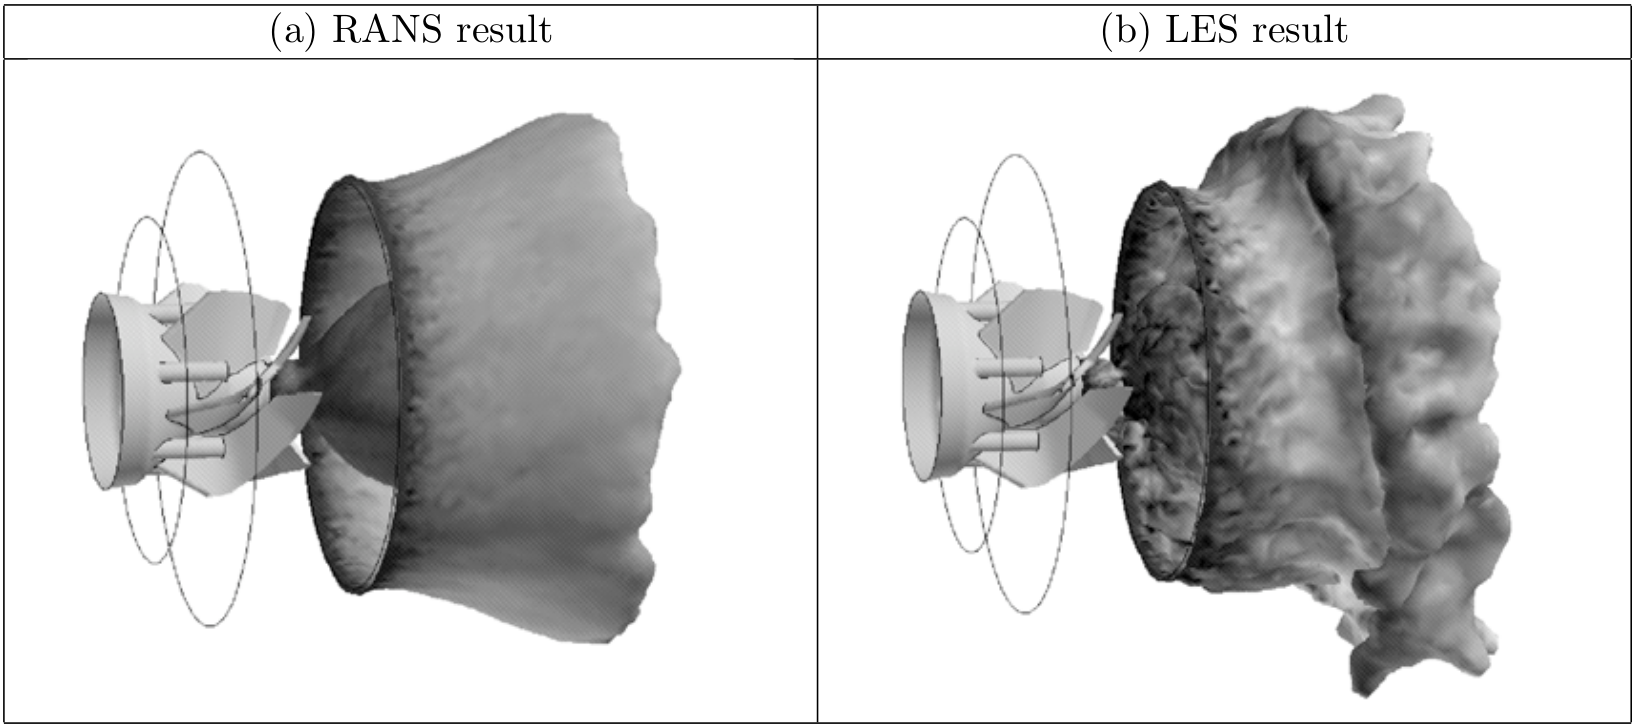
\includegraphics[width=\textwidth]{figures/rans_vs_les.png}
    \caption{Comparison of temperature isosurfaces in a swirled combustor when
    using \ac{RANS} and \ac{LES}. Image source: Poinsot and Veynante
    \cite{Poinsot2012}}
    \label{fig:rans_vs_les}
\end{figure}
%
Computational fluid dynamics (\acs{CFD}\acused{CFD}) knows three main categories
of models for simulating turbulent flow.
%
They are, in decreasing order of abstraction, \acf{RANS}, \acf{LES} and
\acf{DNS}.
%
For simulating turbulent combustion, these are extended by combustion models
according to their character.
%
\Cref{part:flame_vis} of this thesis focuses heavily on \ac{DNS}, which is
discussed in detail in the next section.
%
Since \ac{DNS} is one of the main tools for validating and building \ac{RANS}
and \ac{LES} models, we will briefly discuss the ideas behind both here.
%
\subsubsection{Reynolds-Averaged Navier-Stokes} % (fold)
\label{ssub:rans}
%
\acl{RANS} equations describe the time-averaged behavior of the system.
%
It is based on the decomposition of a turbulent flow into mean and
fluctuating parts.
%
The result are average values for all simulation variables at each location.
%
Images of \ac{RANS} simulations show very smooth fields that have almost no
small-scale features (see \eg, \cref{fig:rans_vs_les}).
%
The typical \ac{RANS} equations assume a steady-state system, but the \ac{URANS}
variant can account for some unsteady behavior if it is slow compared to the
turbulent timescales.
%

%
Combustion models for \ac{RANS} can be based on quantities such as the mean
flame surface area per unit volume, turbulent mixing rates, or probability
density functions based on one-point statistics.
%

%
Since \ac{RANS} simulations only resolve time-averaged values, their results
have to be interpreted with care.
%
Mean values reported by \ac{RANS} at a certain location say nothing about the
possibly large fluctuations that occur there.
%
However, \ac{RANS} is the most popular and widespread method for simulating
turbulent combustion because of its low computational cost.
%
% subsubsection rans (end)
%
\subsubsection{Large Eddy Simulations} % (fold)
\label{ssub:les}
%
A step up from \ac{RANS} in terms of accuracy and computational cost are
\ac{LES}.
%
They reproduce unsteady, but low-pass filtered effects of the system.
%
The simulation runs on a lower-resolution grid and only resolves the larger
scales explicitly.
%
Small-scale sub-grid effects are modeled.
%
\ac{LES} produce an unsteady, but "blurry" representation of reality (see
\cref{fig:rans_vs_les}).
%

%
Combustion models for \ac{LES} face the challenge that the flame front is
generally much smaller than the grid resolution.
%
Combustion phenomena that control the evolution of the flame front happen almost
exclusively at sub-grid scales.
%
\ac{LES} approaches deal with this by describing the flame front in terms of
some filtered variable that can be resolved on the grid.
%
Some approaches artificially thicken the flame front, others assume the
flame front as an isosurface of some smooth variable.
%
In any case, small-scale wrinkling of the flame front cannot be resolved in
\ac{LES} and needs to be expressed via models.
%

%
With the increase in computing performance in recent years, \ac{LES} has gained
popularity and is seeing more widespread use.
%
However, \ac{LES} of turbulent combustion is still maturing, and accurate
sub-grid models for combustion are the subject of ongoing research.
%
% subsubsection les (end)
%
% subsection high_level_models_for_turbulent_combustion_ac (end)
%
\subsection{Direct Numerical Simulations} % (fold)
\label{sub:direct_numerical_simulations}
%
The most accurate and detailed numerical results in \ac{CFD} are produced by
\ac{DNS}.
%
In these simulations, all time and length scales are resolved on a regular grid.
%
On this grid, the Navier-Stokes equations are solved directly without using a
model for turbulence.
%
This produces an accurate representation of reality, which is why \ac{DNS} is
also often referred to as a ``numerical experiment''.
%

%
Its brute-force approach means that \ac{DNS} is conceptually relatively simple
compared to \ac{RANS} and \ac{LES}, but it is the most demanding of the three
in terms of computational resources and time.
%
As a consequence, \ac{DNS} are typically used only for small domains of a few
centimeters at most.
%
Although methods for more complex setups and geometries are under active
development, the typical case is a rectangular box with simple boundary
conditions.
%
This is why non-reacting \ac{DNS} has typically been used to study turbulent
flows near walls, between parallel plates or behind simple rectangular
geometries.
%

%
Like for \ac{RANS} and \ac{LES}, the choice of a chemistry model for \ac{DNS} is
largely dependent on the available computing resources and performance demands.
%
If we apply the ideal of solving everything without high-level models, then the
logical choice would be using complex chemistry with full chemical schemes.
%
Unfortunately, this is rarely feasible.
%
Even adding single-step chemistry to a non-reacting \ac{DNS} can result in a
hundred-fold increase in computing time due to the smaller time steps and grid
sizes required.
%
Using complex chemical schemes only amplifies this problem.
%
For complex fuels, the only choice for getting results in a reasonable time
frame is therefore to make a massive trade of accuracy in favor of performance.
%
Even then, turbulent combustion \ac{DNS} of non-trivial cases can only be run
on large supercomputers using thousands of parallel cores.
%
See S3D~\cite{Chen2009,Treichler2017} and DINO~\cite{Abdelsamie2016} for two
modern \ac{DNS} codes.
%

%
Despite the large computational cost and restriction to simple case setups,
\ac{DNS} is an important tool for combustion modeling.
%
It provides high-resolution \ac{3D} unsteady data for all variables, which is
still impossible to obtain via experiments.
%
This data allows an in-depth analysis of the behavior of turbulent flames that
can be leveraged to build, validate and improve higher-level models.
%
\begin{figure}[t]
    \centering
    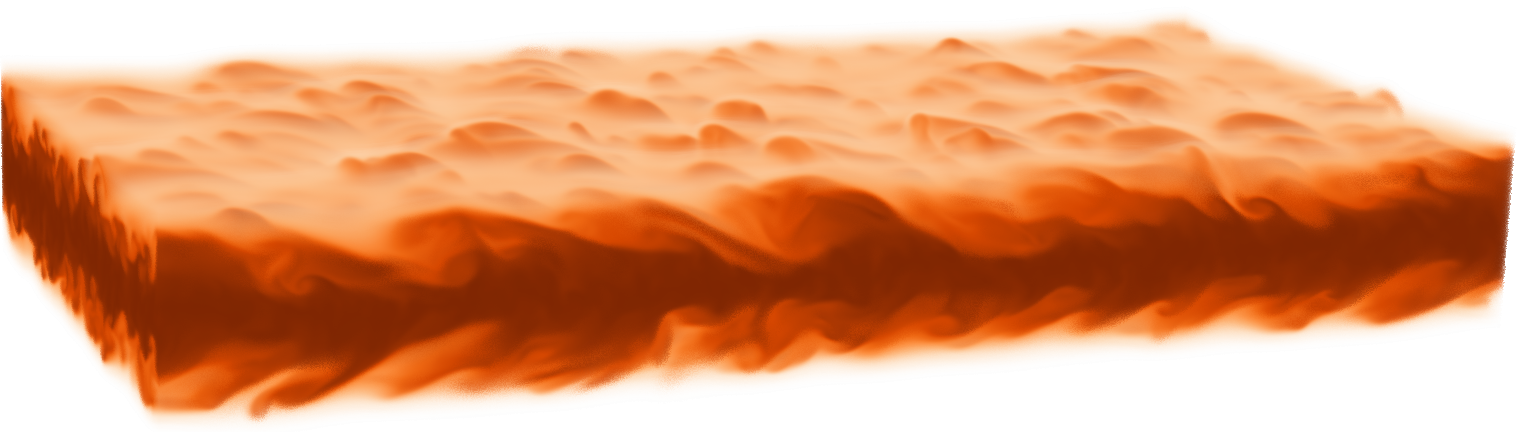
\includegraphics[width=\textwidth]{figures/Hawkes_VolRend.png}
    \caption{Direct volume rendering of the mixture fraction in a
    \ac{DNS} of a turbulent non-premixed flame.}
    \label{fig:turbulent_diffusion_flame_dns}
\end{figure}
%

%
\ac{DNS} is used mainly for two purposes:
%
Gaining data to validate and fine-tune \ac{RANS} and \ac{LES} models, and
gaining a deeper understanding of turbulence/chemistry interactions to derive
new models.
%
A wide variety of analysis approaches are applied to these effects.
%
These range from very simple validation by looking at aggregated quantities to
investigation of complex effects such as the different mechanisms for
re-ignition of locally extinguished parts of the flame.
%
Providing an exhaustive discussion would go beyond the scope of this chapter,
but we will take a look at some examples to get an idea of the kind of
properties that are investigated.
%

%
The simplest forms of analysis are applied for the validation of \ac{RANS} and
\ac{LES} models.
%
Here, the same case is simulated once using \ac{RANS} or \ac{LES}, and once
using \ac{DNS}.
%
Validation can happen at a high level by comparing aggregated quantities such as
the average or maximum temperatures, or on a lower level by comparing point-wise
quantities or statistics.
%
In this case it is important to take into account the differences in
representation between \ac{DNS} and the higher-level models.
%
In the case of \ac{RANS}, \ac{DNS} results have to be temporally averaged in
order to be meaningfully comparable.
%
For \ac{LES}, the \ac{DNS} data needs to be low-pass filtered before comparison.
%

%
More complex analysis is needed when checking the validity of basic assumptions
underlying the high-level models, such as the flamelet assumption.
%
In the case of \ac{RANS}, this can be done by computing different kinds of
statistics, depending on the combustion model used.
%
Simple point statistics can be computed without regard for the flame structure.
%
If the flame front is thin, flamelets may be extracted as profiles orthogonal
to an isosurface representing the flame surface, or along trajectories of the
temperature or mixture fraction gradient.
%
Statistics may also be derived from ensembles of iso-levels of characteristic
variables such as temperature or mixture fraction.
%
The result are distributions as a function of this variable.
%
Finally, space-averaged statistics might be used to determine quantities such as
the average amount of flame surface area per unit volume.
%

%
Other quantities that are often investigated due to their significance in
combustion modeling are the flame speed (if applicable), thickness, surface
stretch and curvature.
%
The relationship of all of these quantities with the structure of the flame is
still not completely understood.
%
This is why \ac{DNS} results are frequently compared to laminar flames as a
baseline.
%
For example, Sankaran \etal{}~\cite{Sankaran2007} analyzed the flame thickness and
curvature in a premixed jet flame statistically and compared the results to a
laminar flame.
%
Hawkes and Chen~\cite{Hawkes2006} investigated the statistical similarity of
methane-air flames in the ``thin reaction zones'' regime, which uses slightly
weaker assumptions than the flamelet regime, to strained laminar flames.
%
The approach presented in \cref{cha:sparse_representation} facilitates such
studies by providing a representation of a premixed flame from which such
statistics can readily be computed, as well as enhancing it by an additional
possibility of visual analysis.
%

%
A promising area of current research is concerned with the mechanisms of local
extinction and re-ignition and the effect of unsteady, non-instantaneous effects
on the flame.
%
These are especially interesting for diffusion flames, as they are more
sensitive to turbulence and local extinction has a major significance for the
applicability of flamelet models.
%
Many works in this area use Lagrangian approaches to study the temporal behavior
of flame elements.
%

%
Yeung \etal{}~\cite{Yeung1990} tracked ensembles of points attached to material-
and flame surfaces in premixed and diffusion flames.
%
They recorded the histories of strain rates acting on these surface points to
determine under what circumstances a flame surface remains close to an initially
coincident material surface.
%
Statistics extracted from the ensemble of surface points allowed them to
determine in what way the flame surface grows or shrinks over time and how the
strain experienced by a flame surface element affects the flame dynamics.
%

%
Sripakagorn \etal{}~\cite{Sripakagorn2004} tracked points attached to an
isosurface of the mixture fraction over time to detect and classify local
extinction and re-ignition events.
%
They showed that extinction happens primarily if the flame surface is subject to
large amounts of strain over a certain time period.
%
They also identified three different mechanisms for re-ignition of previously
extinguished parts of the flame.
%

%
Scholtissek \etal{}~\cite{Scholtissek2017} tracked complete flamelets represented
as trajectories of the mixture fraction gradient emanating from such points on
the mixture fraction isosurface.
%
They analyzed the histories of these flamelets and derived a new flamelet model
that accounts for curvature-induced tangential transport between adjacent
flamelets.
%

%
Such Lagrangian approaches are becoming more prevalent in the combustion
community.
%
They provide an important tool for the derivation of new combustion models
that incorporate unsteady effects.
%
\Cref{cha:flame_surface_tracking} of this thesis presents an approach for
tracking the complete flame surface that is intended to support such
investigations in large-scale \ac{DNS}.
%
% subsection direct_numerical_simulations_for_turbulent_combustion (end)
%
% section modeling_and_simulation_of_turbulent_combustion (end)